% set encoding to UTF-8 Unicode
\documentclass[sigconf]{acmart}
\bibliographystyle{acmart}
%automatically run bibtex
\def\BibTeX{{\rm B\kern-.05em{\sc i\kern-.025em b}\kern-.08emT\kern-.1667em\lower.7ex\hbox{E}\kern-.125emX}}

\copyrightyear{2019}
\acmYear{2019}
\setcopyright{acmlicensed}
\acmConference[UWT '19]{UWT '19: TCSS 555: Machine Learning}{Winter 2019}{Tacoma, WA}
\acmPrice{0.00}
\acmDOI{10.1145/1122445.1122456}
\acmISBN{978-1-4503-9999-9/18/06}

\begin{document}
%
% paper title
% can use linebreaks \\ within to get better formatting as desired
\title{Predicting Malware Detection Using Machine Learning Methods}

\author{Jeffrey Lytle}
\authornote{Both authors contributed equally to this research.}
\email{jjlytle@uw.edu}
\orcid{1234-5678-9012}
\author{Jason Hall}
\authornotemark[1]
\email{b29@uw.edu}
\affiliation{%
  \institution{University of Washington}
  \streetaddress{1900 commerce st.}
  \city{Tacoma}
  \state{Washington}
  \postcode{98001}
}

\begin{abstract}
 The goal of this study is to find an optimal solution using machine learning methods to develop a model that will efficiently predict malware detection given parameters described later. The models described in this study were trained on a dataset created by Microsoft.  
\end{abstract}

\begin{CCSXML}
<ccs2012>
<concept>
<concept_id>10002978.10002997.10002998</concept_id>
<concept_desc>Security and privacy~Malware and its mitigation</concept_desc>
<concept_significance>300</concept_significance>
</concept>
<concept>
<concept_id>10010147.10010257</concept_id>
<concept_desc>Computing methodologies~Machine learning</concept_desc>
<concept_significance>500</concept_significance>
</concept>
<concept>
<concept_id>10010147.10010341</concept_id>
<concept_desc>Computing methodologies~Modeling and simulation</concept_desc>
<concept_significance>400</concept_significance>
</concept>
<concept>
<concept_id>10002944.10011122.10002946</concept_id>
<concept_desc>General and reference~Reference works</concept_desc>
<concept_significance>100</concept_significance>
</concept>
</ccs2012>
\end{CCSXML}

\ccsdesc[300]{Security and privacy~Malware and its mitigation}
\ccsdesc[500]{Computing methodologies~Machine learning}
\ccsdesc[400]{Computing methodologies~Modeling and simulation}
\ccsdesc[100]{General and reference~Reference works}


\keywords{Malware, Machine Learning, Support Vector Machines (SVM), Random Forest, Logistic Regression, Malware Detection, Microsoft, Deep Learning, Comma Separated Value (CSV)
}

\begin{teaserfigure}
  
\includegraphics[width=\textwidth]{malware}
  \caption{Malware is all malicious software.}
  \label{fig:teaser}
\end{teaserfigure}

%Everything above here is for the title bar Main text below
\maketitle

\section{Introduction}
 The problem this study attempts to address is the problem of malware on computers. What is malware? Malware is any software intentionally designed to cause damage to a computer, server, client, or computer network. \cite{cite-Moir:2009}. Malware is actually short for 'Malicious Software'. The problem is how can one prevent computers from ever acquiring these programs. What makes a computer vulnerable to acquiring malware? This study looks at a data set of 8,029,335 data points each with 83 features. \textit{Some unknown number of data points were kept secret for testing.} Each data point in this dataset represents a physical computer and whether or not this computer has had a malware detection. The features of this dataset represent the states of a physical computer, such as how much RAM it has, or whether or not automatic updates were on or off. As well as details about which OS and OS build were installed on the computer. With these and the other ~80 features we attempted to build a machine learning model that could predict with some accuracy as to whether or not the machine in question is predicted to be infected with malware. This study details the methods and experiments carried out to build an optimal model for this problem of detecting malware.

\section{Background}
This study was used as an introduction to machine learning in the \textit{University of Washington Tacoma's (UWT) Winter 2019 TCSS 555 Machine Learning class.} The data was broken into two sections, one given to the students and one reserved for testing and grading by the professor. The dataset given to the students was around 8 million rows and the test dataset size was unknown. The testing was also resource constrained. The testing was done on a x84\_64 AMD Ryzen Threadripper 1950X 16-Core Processor at 3393.566 MHz using a virtualized Linux environment using the KVM hypervisor. With 8167936 KB of memory, but only 7584916 KB of memory was available to the processes. The L1\_d cache was 32K, L1\_i cache was 64K, L2 was 512K, and L3 was 32768K bytes. This CPU has 4 cores with one thread per core. The resource constraints, unknown data, and unknown data size were major factors in the data preprocessing as well as model training. Model training itself was unconstrained and models could be built on any compatible system and then uploaded to the test system described above. 
 
\section{Dataset and Metrics}
This dataset was provided by Microsoft for their 2015 Malware Classification Challenge (BIG 2015). The dataset contains state information about physical computers. The target feature we are most interested is `HasDetection' this binary value indicates whether the physical computer has detected some form of malicious software when in its current state. We used the state information contained in the dataset to train models to predict the target feature 'HasDetection'. The Metric we used to optimize the models was Area Under the Curve (AUC) Receiver Operating Characteristics (ROC) curve. AUC - ROC curve is a performance measurement for classification problem at various thresholds settings. ROC is a probability curve and AUC represents degree or measure of separability. It tells how much model is capable of distinguishing between classes. The higher the AUC, the better the model is at predicting 0s as 0s and 1s as 1s. \cite{AUC:2018} The ROC curve is a plot of True Positive Rate (TPR) vs. the False Positive Rate (FPR). Thus AUC is the area under the TPR vs. FPR curve. Most models were trained for accuracy in predicting `HasDetection' then compared by their average AUC.

 \begin{figure}
  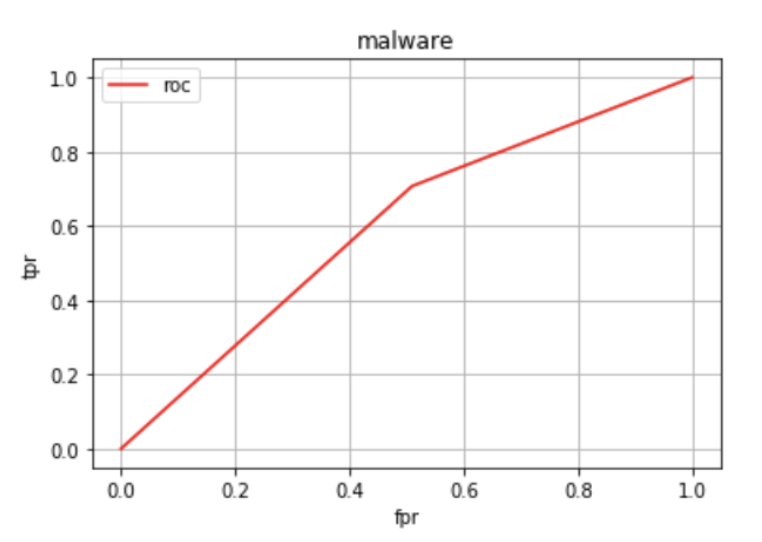
\includegraphics[width=\linewidth]{example-ROC.PNG}
  \caption{Example Receiver Operating Characteristics Curve.}
  \label{fig:roc}
\end{figure}

\begin{equation}
\text { TPR / Recall / Sensitivity }=\frac{\text { TP }}{\mathrm{TP}+\mathrm{FN}}
\end{equation}

\begin{equation}
\text { Specificity }=\frac{\text { TN }}{\mathrm{TN}+\mathrm{FP}}
\end{equation}

\begin{equation}
\begin{aligned} \mathrm{FPR} &=1-\text { Specificity } \\ &=\frac{\mathrm{FP}}{\mathrm{TN}+\mathrm{FP}} \end{aligned}
\end{equation}
 
\section{Data Analysis}:
For this study we were given a dataset in the form of a .csv file. This data was collected by Microsoft and contains many statistics about individual physical computers. The first step in all machine learning studies is looking at the dataset and attempting to gain a general understanding of the information it contains. 
\subsection{Feature Selection Models}
This dataset contains some 80 odd features. The first thing we did was look through the data and try to obtain a general understanding of the information contained in our dataset, also looking at what malware is and how it affects a computer. We looked at the features and used our intuition as to whether or not this feature would be useful in detecting malware. We choose a list of ten features we thought would contain the most useful information for detecting malware. 
% so we start with a simple list
\subsubsection{Initial Tests}
We chose this smaller set of features to allow models to be trained quickly so that when setting up the training and testing environment we would have no issue with the testing's resource constraints. This would allow us to get an initial baseline. This initial set will be added to and subtracted from to form a final list of features. This initial list was used to set up the testing and training environment quickly so we could get to iterating
\begin{center}
\textbf{`Firewall':}\\
    \textbf{\textit{Datatype: }}int8\\
    \textbf{\textit{Definition: }}Bit is set if windows firewall is enabled. \\
    \textbf{\textit{Intuition: }}Computers are much more vulnerable to malware with the firewall off.\\
    \vspace{5mm}
    \textbf{`IsProtected'):\\}
    \textbf{\textit{Datatype: }}float16\\
    \textbf{\textit{Definition: }}True if active up-to-date antivirus product, False if no active AV product, null no AV. \\
    \textbf{\textit{Intuition: }}Up-to-date antivirus definitions should play a major role in whether a system is vulnerable to malware infection.\\
    \vspace{5mm}
    \textbf{`Census\_OSWUAutoUpdateOptionsName':\\}
    \textbf{\textit{Datatype: }}int8\\
    \textbf{\textit{Definition: }}Friendly name of the WindowsUpdate auto-update settings on the machine. \\
    \textbf{\textit{Intuition: }}Computers are much more vulnerable to malware with the auto update options switched off.\\
    \vspace{5mm}
    \textbf{`Census\_GenuineStateName':\\}
    \textbf{\textit{Datatype: }}categorical\\
    \textbf{\textit{Definition: }}Category is set to 0 if the installed copy of windows was a genuine copy of windows another number otherwise.\\
    \textbf{\textit{Intuition: }}Non genuine copies of windows typically have malware installed on them from the start.\\
    \vspace{5mm}
    \textbf{`Census\_ActivationChannel':\\}
    \textbf{\textit{Datatype: }}categorical\\
    \textbf{\textit{Definition: }}Retail license key or Volume license key for a machine. \\
    \textbf{\textit{Intuition: }}A volume license key means a professional installed the OS where a retail license means a non professional installed the OS, This may introduce a line of attack due to default or improper settings.\\
    \vspace{5mm}
    \textbf{`Census\_IsAlwaysOnAlwaysConnectedCapable':\\}
    \textbf{\textit{Datatype: }}float16\\
    \textbf{\textit{Definition: }}Retrieves information about whether the battery enables the device to be AlwaysOnAlwaysConnected. \\
    \textbf{\textit{Intuition: }}This setting allows the computer to connect to any available WiFi even when closed or asleep. If this is set incorrectly it is a very good attack vector for malware.\\
    \vspace{5mm}
    \textbf{`DefaultBrowsersIdentifier':\\}
    \textbf{\textit{Datatype: }}float16\\
    \textbf{\textit{Definition:}}ID for the machine’s default browser.\\
    \textbf{\textit{Intuition: }}An old or out-of-date browser could be a potential attack vector for malware.\\
    \vspace{5mm}
    \textbf{`ProductName':\\}
    \textbf{\textit{Datatype: }}category\\
    \textbf{\textit{Definition: }}Defender state information e.g.  win8defender. meaning name of installed antivirus\\
    \textbf{\textit{Intuition: }}The installed antivirus should have a major impact as to whether a system is infected with malware, as not all antivirus programs are equal in how they defend against malware.\\
    \vspace{5mm}
    \textbf{`Platform':\\}
    \textbf{\textit{Datatype: }}category\\
    \textbf{\textit{Definition: }} Calculates platform name. This is a friendly name for the installed OS.\\
    \textbf{\textit{Intuition: }}Every OS deals with program permission and instillation different, Linux typical has very low occurrences of malware where Windows XP is famous for its malware infections\\
    \vspace{5mm}
    \textbf{`SkuEdition':\\}
    \textbf{\textit{Datatype: }}category\\
    \textbf{\textit{Definition: }}The ’SKU-Edition’ is a string value that is in one of three classes of results. \\
    \textbf{\textit{Intuition: }}This specifies if the OS edition Home, Pro, Enterprise, Education or invalid (OS other than Windows). Malware may attack Enterprise and Education as large business regularly pay off ransom wear attacks\\
    \vspace{5mm}
    \textbf{`SMode':\\}
    \textbf{\textit{Datatype: }}int8\\
    \textbf{\textit{Definition: }}S Mode’, where only specific apps can be installed \\
    \textbf{\textit{Intuition: }}S mode of safe mode is a mode windows has where only digitally signed apps can be signed. This added security should make it harder for malware to install itself\\
    \vspace{5mm}
\end{center}
% re-encoded the data
After we got a good handle on what the data contained and why it would be used to detect malware. We moved on to looking at the data mathematically. 
\subsubsection{Re-encoding to Reduce Memory Footprint}
This is where we hit our first hurdle. Due to the resource constraints imposed on this problem, we needed to reduce the memory footprint of the information contained in the dataset. We achieved this by re-encoding the default datatypes passed to the training model and testing environment. In the dataset, some binary values are encoded as floats, so 1, 0 were encoded as 1.0, 0.0. This takes up a lot of memory and provides no extra information. These are the simple rules we used for re-encoding the data so it would take up less physical memory without losing any information:
\begin{itemize}
\item python's 'object'$\,\to\,$pandas category
\item all Binary values$\,\to\,$int8
\item Binary values with missing values$\,\to\,$float16 (int8 does not understand NaN).
\item 64 bits encoding$\,\to\,$float32, or float16 if possible
\end{itemize}

This re-encoding of the data allowed for quicker manipulations to the structure of the data and allowed for the model to be trained on the entire dataset when this, and other tricks were used (discussed later). 
 % then we look at Pearsons correlations
 \subsubsection{Using the Pearson's Correlation to Select Features}
 The next thing we did was produce a correlation matrix (see appendix [1] for full size). 
 \begin{figure}
  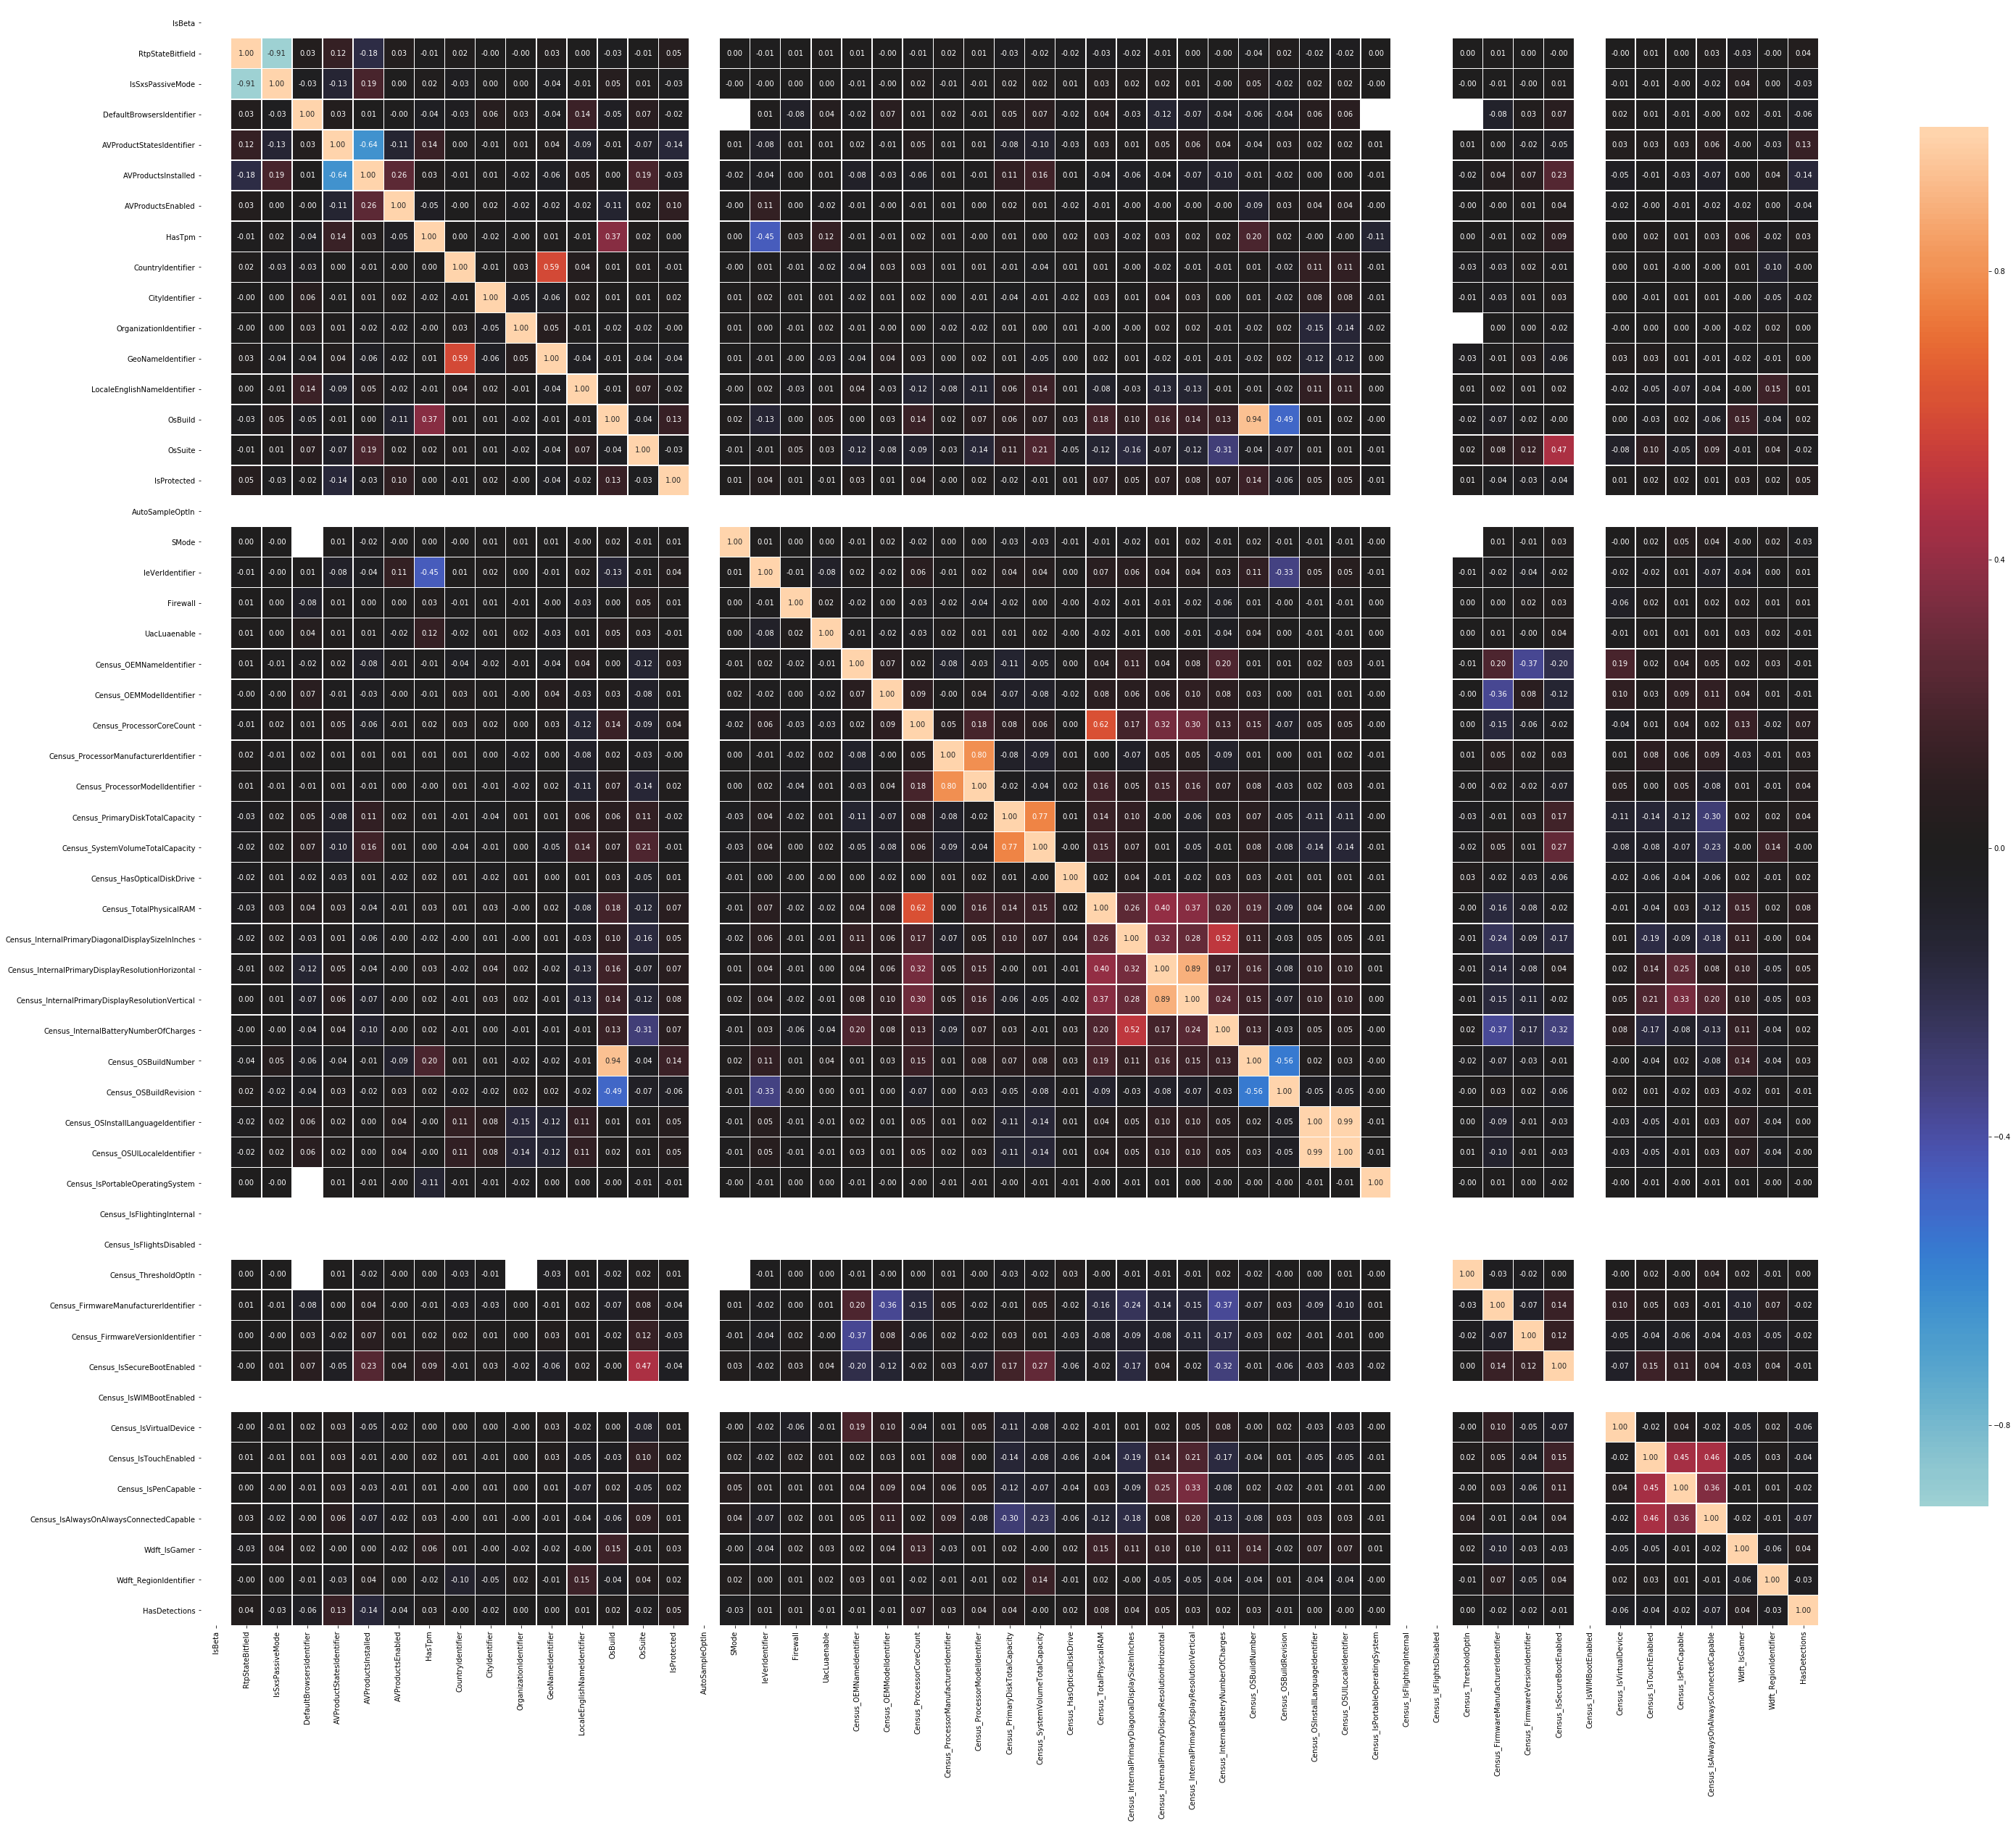
\includegraphics[width=\linewidth]{correlation.PNG}
  \caption{Pearson Correlation Matrix}
  \label{fig:matrix}
\end{figure}

Figure \ref{fig:matrix} This matrix was made using Pearson's correlation. 

\begin{equation}
r=\frac{\sum(x-\overline{x})(y-\overline{y})}{\sqrt{\sum(x-\overline{x})^{2} \sum(y-\overline{y})^{2}}}
\end{equation}

 The matrix shows the correlation of every feature with every other feature in the dataset. This allowed us to see which features where highly correlated with the data and which features were highly correlated with each other. 
% drops do to correlation 
 This allowed us to quickly decide to drop columns that were highly correlated with each other. This is because features that equal ~1 using Pearson's contain the same information, so when training models this feature will provide no new information while taking up precious memory in our resource constrained system. The columns we decided to drop that had too high a correlation with each other were:

\begin{center}
\textbf{`Census\_OSBuildNumber':}\\
    \textbf{\textit{Feature Removed: }}`OSBuild'\\
    \textbf{\textit{Definitions:}} Both OSBuild and Census\_OSBuildNumber represent the build of the OS, but OSBuildNumber is slightly more specific so OSBuild feature was removed.\\
    \textbf{\textit{Correlation: }}94\%.\\
    \vspace{5mm}
\textbf{`IsSxsPassiveMode':}\\
    \textbf{\textit{Feature Removed: }}`RtpStateBitfield'\\
    \textbf{\textit{Definitions:}} IsSxsPassiveMode is set if your firewall is set to active or passive mode. RtpStateBitfield states whether your firewall has real-time protection enabled or disabled, Real time protection sets your firewall from active to passive modes so these bits should always be in sync. The correlation is not 100\% due to some missing values.\\
    \textbf{\textit{Correlation: }}91\%.\\
    \vspace{5mm}
\textbf{`Census\_OSInstallLanguageIdentifier':}\\
    \textbf{\textit{Feature Removed: }}`Census\_OSUILocaleIdentifier'\\
    \textbf{\textit{Definitions:}} Census\_OSInstallLanguageIdentifier is used Census\_OSUILocaleIdentifier by default and are almost never changed. \\
    \textbf{\textit{Correlation: }}99\%.\\
    \vspace{5mm}
\textbf{`Census\_InternalPrimaryDiagonalDisplaySizeInInches':}\\
    \textbf{\textit{Feature Removed: }}`Census\_InternalPrimaryDisplayResolutionHorizontal' and \\
    `Census\_InternalPrimaryDisplayResolutionHorizontal'
    \textbf{\textit{Definitions:}} Although not highly correlated using reason one could deduce that A screens horizontal and vertical resolution is correlated with its diagonal display size, therefore we would be using memory in our machine learning model to deduce if a screens aspect ration makes it vulnerable to malware. Which is clearly not true.\\
    \textbf{\textit{Correlation: }}80\%.\\
    \vspace{5mm}
\textbf{`Census\_SystemVolumeTotalCapacity':}\\
    \textbf{\textit{Feature Removed: }}`Census\_PrimaryDiskTotalCapacity'\\
    \textbf{\textit{Definitions:}} Although not highly correlated one could reason that since Census\_PrimaryDiskTotalCapacity  is contained in Census\_SystemVolumeTotalCapacity, so no new information would be found because the primary disk capacity is part of the total system capacity. For this reason it was removed\\
    \textbf{\textit{Correlation: }}79\%.\\
    \vspace{5mm}
\end{center}

Using this same correlation matrix, we can see how each feature is correlated to our target `HasDetection’, which is the feature we are trying to predict. `HasDetection' indicates that the physical computer this datapoint represents has detected a known malicious program in the past. We decided to keep the top X most positively and negatively correlated features. Those features were:

\begin{center}
\begin{tabular}{ |c|c| } 
 \hline
 Feature & Pearson's correlation \\
  \hline\hline
 AVProductsInstalled & -0.103090 \\
  \hline
Census\_IsPenCapable & -0.078027 \\
 \hline
Census\_FirmwareVersionIdentifier & -0.071773 \\
 \hline
Census\_IsTouchEnabled & -0.063520 \\
 \hline
AVProductsEnabled & -0.062365 \\
 \hline
Census\_OSUILocaleIdentifier & -0.058779 \\
 \hline
Census\_ProcessorCoreCount & 0.072079 \\
 \hline
Census\_PrimaryDiskTotalCapacity & 0.082228 \\
 \hline
Census\_ProcessorModelIdentifier & 0.093179 \\
 \hline
AVProductStatesIdentifier & 0.098968 \\
 \hline
Census\_ProcessorManufacturerIdentifier & 0.099886 \\
 \hline
\end{tabular}
\end{center}
\vspace{3mm}

The next data preprocessing task was to find and remove highly skewed columns, as well as empty columns and columns that contained unique values for every entry. We removed data where either all entries were equal or very close to equal. The dataframes .skew() function was used to obtain the Pearson's skew of the columns, which defines skew as the mean minus the mode divide by the standard deviation. This means that any column whose skew is zero or very close to it contains mostly the same values. We also used the pandas dataframe's .value\_count to obtain the number of unique values in a column. Any column whose value count was equal to the size of the dataframe where removed. This means that every value in the column was unique and thus could provide no value to our machine learning model and would take up constrained memory. These are the features that were removed using this process:

\begin{center}
\begin{tabular}{ |c|c|c| } 
 \hline
 Feature & Reason Dropped \\
 \hline\hline
IsBeta & All entries are equal \\
AutoSampleOptIn & All entries are equal \\
Census\_IsFlightingInternal & over 95\% missing \\
Census\_IsFlightsDisabled & All entries are equal \\
Census\_IsWIMBootEnabled & over 95\% missing \\
Census\_ThresholdOptInv & All entries are equal \\
Census\_IsFlightsDisabled & All entries are equal \\
AutoSampleOptIn & All entries are equal \\
CityIdentifier & highly skewed \\ 
 \hline
\end{tabular}
\end{center}
\vspace{3mm}

This left us with a final list of 27 features containing mostly binary features, a few categorical features, and a couple continuous value features. The final feature list started with the 10 most highly correlated features plus the 10 features that would logically pertain to malware detection. This left us with 20 columns. To this initial list we continued to add features starting with the next most highly correlated (excluding those mentioned above as excluded) until we reached the limit of our testing environments resource constraints. This is the final resource list we trained our models with:

\begin{itemize}
\item `AVProductsInstalled' 
\item `Census\_IsAlwaysOnAlwaysConnectedCapable',
\item `DefaultBrowsersIdentifier',
\item `ProductName',
\item `Platform',
\item `SkuEdition',
\item `IsProtected',
\item `Firewall',
\item `Wdft\_IsGamer',
\item `Census\_OSWUAutoUpdateOptionsName',
\item `Census\_GenuineStateName',
\item `Census\_ActivationChannel',
\item `Census\_ProcessorCoreCount',                               
\item `Census\_TotalPhysicalRAM',                             
\item `AVProductStatesIdentifier',
\item `Census\_IsVirtualDevice',
\item `Census\_IsTouchEnabled',
\item `AVProductsEnabled',
\item `SMode',
\item `Wdft\_RegionIdentifier',
\item `IsSxsPassiveMode',
\item `Census\_IsPenCapable',
\item `OsSuite',
\item `Census\_FirmwareManufaturerIdentifier',
\item `Census\_FirmwareVersionIdentifier',,
\item `UacLuaenable',
\item `Census\_OSBuildRevision',
\end{itemize}

\section{Methodology}
Now that we have a handle on the data and have removed all irrelevant and extraneous data, we will talk about our model training methodology.  We chose to use a typical machine learning model selection methodology starting with linear regression. Then we would check results, move to logistic regression, and check results again. Next, we would try random forest. These failing, we would then begin trying more exotic methods. Our initial test failed to produce good results, so we attempted SVM and deep learning methods due to some research articles into the dataset that was provided. Before we could train our models, we again were faced with memory constraints.
\subsection{Dealing With Memory Constraints}
When training a model it is best to use as much data as possible. Due to the testing environment, all data manipulation done to the data must also be replicated in the testing environment. This was due to the test environment accepting only a serialized python class as an input. Since only the class is saved, all manipulation to the data done before training the model must also be done to the test data. Due to the fact that model training was not constrained and model testing was, we settled on the process described below to allow our models to be trained on all the data, even when the testing environment could not handle the data manipulations needed for the trained models. First we retrieved the parameters of our test system, such as OS used, Hypervisor used, and other necessary parameters. With these, we created a duplicate virtualized environment, but with much more memory available. We then used this system to train the models and save the serialized class. This class is sent to the resource constrained testing environment. The test system then loads the serialized class and passes it a test-data set in a pandas dataframe and calls the classes predict method. The output of this method is a list object of malware predictions for the test-data this is then compared with the ground truth of the malware predictions to calculate the AUC-ROC graph. We solved the problem of duplicating the test-data transformations to match the model by having the predict method retrieve the entire data frame and re-encode it using these rule:
\begin{itemize}
\item python's 'object'$\,\to\,$pandas category
\item all Binary values$\,\to\,$int8
\item Binary values with missing values$\,\to\,$float16 (int8 does not understand NaN).
\item 64 bits encoding$\,\to\,$float32, or float16 if possible
\end{itemize}
We then write the entire dataframe to a .csv file. We then read the .csv file back, but in chucks of 1000 datapoints a piece. The predict method would then do the data transformations and predictions 1000 datapoints at a time, keeping the entire code well within the memory limits of the test system. Next we will discuss the data transformation we chose to do before training the data.
\subsection{Dealing with missing values}
Due to the high number of missing values contained in the dataset and the fact that most variables were either binary or of a few categories, we decided to implement the pandas imputer class to replace the missing values, such as unknown, blank, or NaN in the dataset with the most frequent value found in the column.
\subsection{Dealing with Categorical values}
Instead of deciding to replace categorical variables with numerical values, we opted to use a method known as one-hot-encoding, a process where each category in a column is given a new column of its own where the data is 0 if the category was different to the new or 1 if the category in the original column matched value of the new column. We used the pandas get\_dummies function to produce this one-hot-encoding. Although this is the easiest method to use when one-hot-encoding the data, it has one potential draw back. It looks at the categorical values and makes a column for each category it finds in a feature. The problem with this is that when we test out model we use only chunks of test data that may not contain all of the possible values a feature could have. This causes get\_dummies to return a transformed test set that has fewer columns than the model was trained on. To counter act this when the model is trained, it saves a list of all feature used to train the model. Then when the predict method is called from the serialized class, it can iterate through the dataframes columns and add a blank column in for any column that was not contained in the test-data chunk. The predict method is also smart enough to remove a column created from a category that was not in any of the training data.
\subsection{Normalizing}
For the few continuous value features, we used standard algebraic normalization. This finds the min and max values and adjusts the values of the feature so that it is continuous between 0 and 1 instead of the min and max of the feature. We used sklearn’s built model normalization form each model’s class.
\begin{equation}
z_{i}=\frac{x_{i}-\min (x)}{\max (x)-\min (x)}
\end{equation}

\subsection{Models Used}
Our model methodology is loosely adopted from How to Choose Algorithms for Azure Machine Learning Studio \cite{order:2019} as this is a good order with which to try and test models.
\begin{itemize}
\item Linear Regression’$\,\to\,$Logistic Regression
\item Logistic Regression$\,\to\,$Random Forest
\item Random Forest$\,\to\,$SVM
\item SVM$\,\to\,$DeepLearning
\end{itemize}
\subsubsection{Linear Regression}
In our very early test, we used the linear regression class from the sklearn package. We trained this model using sum of mean squared error as the cost metric. We tried different combinations of columns with little success. We never achieved more than 0.51 AUC., essentially a coin flip.
\begin{equation}
y=\beta_{0}+\beta_{1} x_{1}+\beta_{2} x_{2}+\ldots+\beta_{n} x_{n}
\end{equation}

\begin{equation}
y \text { is the response }
\end{equation}
\begin{equation}
\beta \text { values are called the model coefficients }
\end{equation}
\begin{equation}
\beta 0 \text { is the intercept }
\end{equation}
\begin{equation}
\beta 1 \text { is the coefficient for } X 1 \text { (the first feature) }
\end{equation}
\begin{equation}
\beta n \text { is the coefficient for } X n \text { (the nth feature) }
\end{equation}

\begin{equation}
\sqrt{\frac{1}{n} \sum_{i=1}^{n}\left(y_{i}-\hat{y}_{i}\right)^{2}}
\end{equation}

 \begin{figure}
  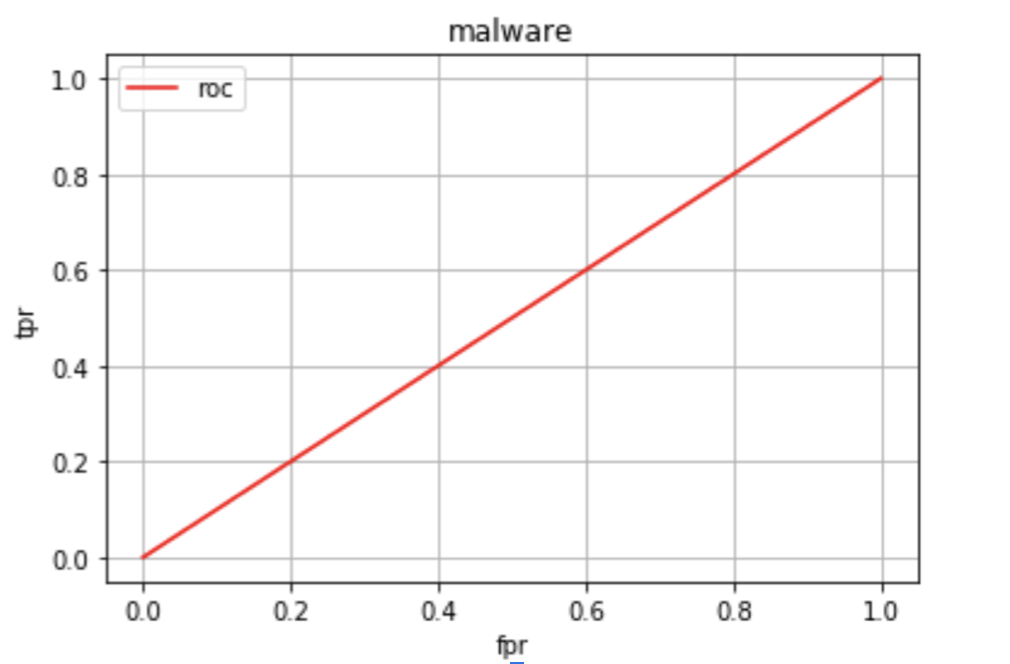
\includegraphics[width=\linewidth]{linear.PNG}
  \caption{Example AUC from linear regression}
  \label{fig:linear}
\end{figure}

\subsubsection{Logistic Regression}
Logistic regression is unlike linear regression, which outputs continuous number values. Logistic regression transforms its output using the logistic sigmoid function to return a probability value \cite{logic:2019}. We did not have any better results with logistic regression than we had with linear regression. We used the sklearn.linear\_model class LogisticRegression. We had to increase the default 150 iterations to 1000 to get it to converge, but still our results were poor with this model. This model also used sum of mean squared error.
\begin{equation}
S(z)=\frac{1}{1+e^{-z}}
\end{equation}
\begin{equation}
s(z)=\text { output between } 0 \text { and } 1 \text { (probability estimate) }
\end{equation}
\begin{equation}
z=\text { input to the function m x+b }
\end{equation}
\begin{equation}
e=\text { base of natural log }
\end{equation}
\subsubsection{Random Forest}
Random forest is a supervised learning algorithm. This algorithm creates many decisions and merges them together to get more accurate predictions. Random Forest adds additional randomness to the model. While creating the model, instead of searching for the most important feature while splitting a node, it searches for the best feature among a random subset of features \cite{random:2019}. 

 \begin{figure}
  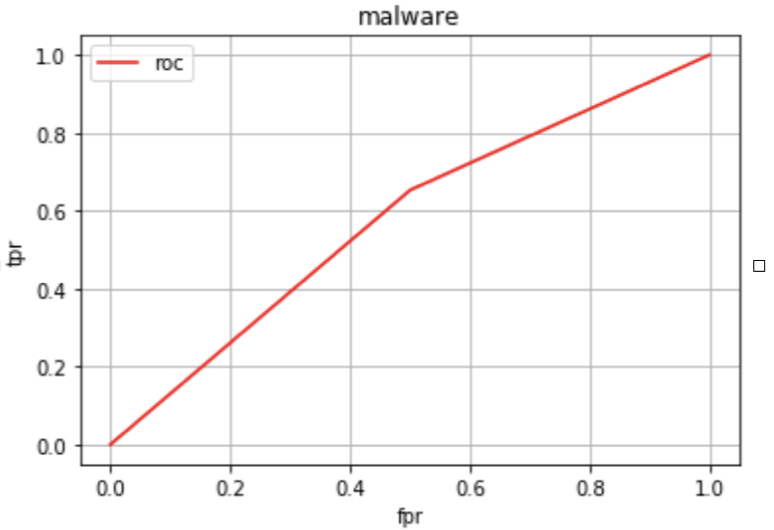
\includegraphics[width=\linewidth]{forest.PNG}
  \caption{Example AUC from Random Forest}
  \label{fig:linear}
\end{figure}

\subsubsection{Support Vector Machines}
Support vector machines are different from other machine learning models in that instead of looking at how features are alike, SVM looks for those datapoints that are most unlike their class and use a vector of these points to create a boundary. The sklearn.svm class SVC can attempt to train on the data with multiple kernels. Kernels are mathematical functions that dictate how these boundaries between the support vectors are drawn. We tried both the linear kernel and the Radial Basis Function (rbf), which is good at solving for datapoints that are isolated and surrounded by a different class. We had slightly better results with the RBF kernel and only an .50 AUC from the linear kernel.

\subsubsection{DeepLearning}
For our deep learning test, we choose the Keras sequential model. The Keras sequential model lets a beginner easily build complex neural networks. Neural networks and all the possible configurations that are possible could be a paper in it self. Due to the time restraints of doing a quarterly project, we could not try or refine our neural networks, but with out simple knowledge we did produce better results than any of the other model types. How we built and trained this model will be discussed in the results section. Neural networks are a computers way of approximating the behavior of the human brain. There are a certain number of input neurons and output neurons. In between the input and out put neurons, there can be any number of hidden layers. These layers can consist of 10 to 1000’s of individual neurons. Each neuron in a layer is connected to the next neuron in the layer. This link also contains a weight. The function of the neurons themselves is typical sigmoid. By using a process known as back propagation, the weights are tweaked until, after applying input to the input neurons and forward propagating, you get the correct prediction. This is known as an epoch. We typically used 100 epochs when training our models.
\section{Results}
The results shown here are the average AUC obtained from 10 runs on test data that was split from the training set. The final AUC is the result we got when we ran our final model on the unknown test data. Due to the limitations of the testing environment, we cannot provide an average AUC for the unknown test data.

\begin{table}[htp]
\caption{default}
\begin{center}
\begin{tabular}{|c|c|}
\hline
Machine Learning Model & Average AUC after 10 iterations \\
\hline\hline
Linear regression & 0.51 \\ 
Logistic Regression & 0.58 \\
SVM Linear Kernel & 0.50 \\
SVM RFB Kernel & 0.60 \\
Keras Sequential & 0.71 \\
\hline
\end{tabular}
\end{center}
\label{default}
\end{table}

For our final test, using our best model, we produced an AUC of 0.69

 \begin{figure}
  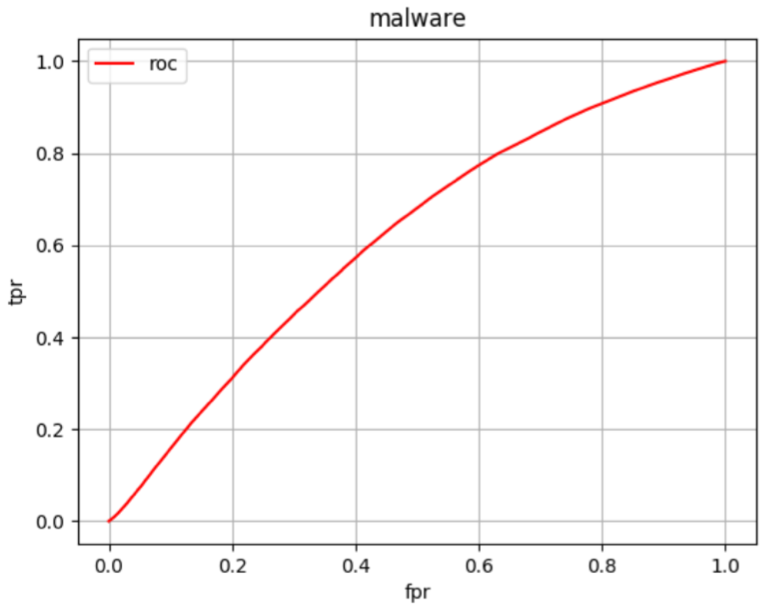
\includegraphics[width=\linewidth]{keras.PNG}
  \caption{Final AUC from Test Set}
  \label{fig:linear}
\end{figure}

This model was built using 8 input neurons. The first hidden layer contained 6 neurons, and the next hidden layer contained 4 neurons and the output only. The activation function on every layer except the output layer was Relu, and the final output’s activations was Sigmoid. 

\begin{equation}
relu = f(x)=\left\{\begin{array}{ll}{0} & {\text { for } x<0} \\ {x} & {\text { for } x \geq 0}\end{array}\right.
\end{equation}

\begin{equation}
sigmoid = S(z)=\frac{1}{1+e^{-z}}
\end{equation}


\section{Conclusions}
As with any project of this magnitude that is done in this short of time span, there are many more things we would like to have tried, experimented with, and learned, but time is a limiting factor in all things. We were slightly happy with our final result, but having that nagging itch of the data scientist, we just want it to be a little better. In conclusion, we do not believe that this data is complete enough or contains enough useful information to truly build an accurate malware predicting model from this data alone. Maybe with some further refinements to the data set and using ensemble or layered learning, one could eke out slightly better results.
\section{Future Work}
In the future, we would like to continue the path of deep learning and experiment with different data transformations as different hyper parameters in the deep learning models. We would like to improve our model enough to submit it to the Microsoft competition. We are also working on a different automated testing environment using AWS cloud resource and an S3 butted with a cloud train log that automatically runs newly uploaded files and emails the result to the sender and the professor. 
\bibliography{main.bib}

\subsection{Appendix}

\label{lytle:correlation}
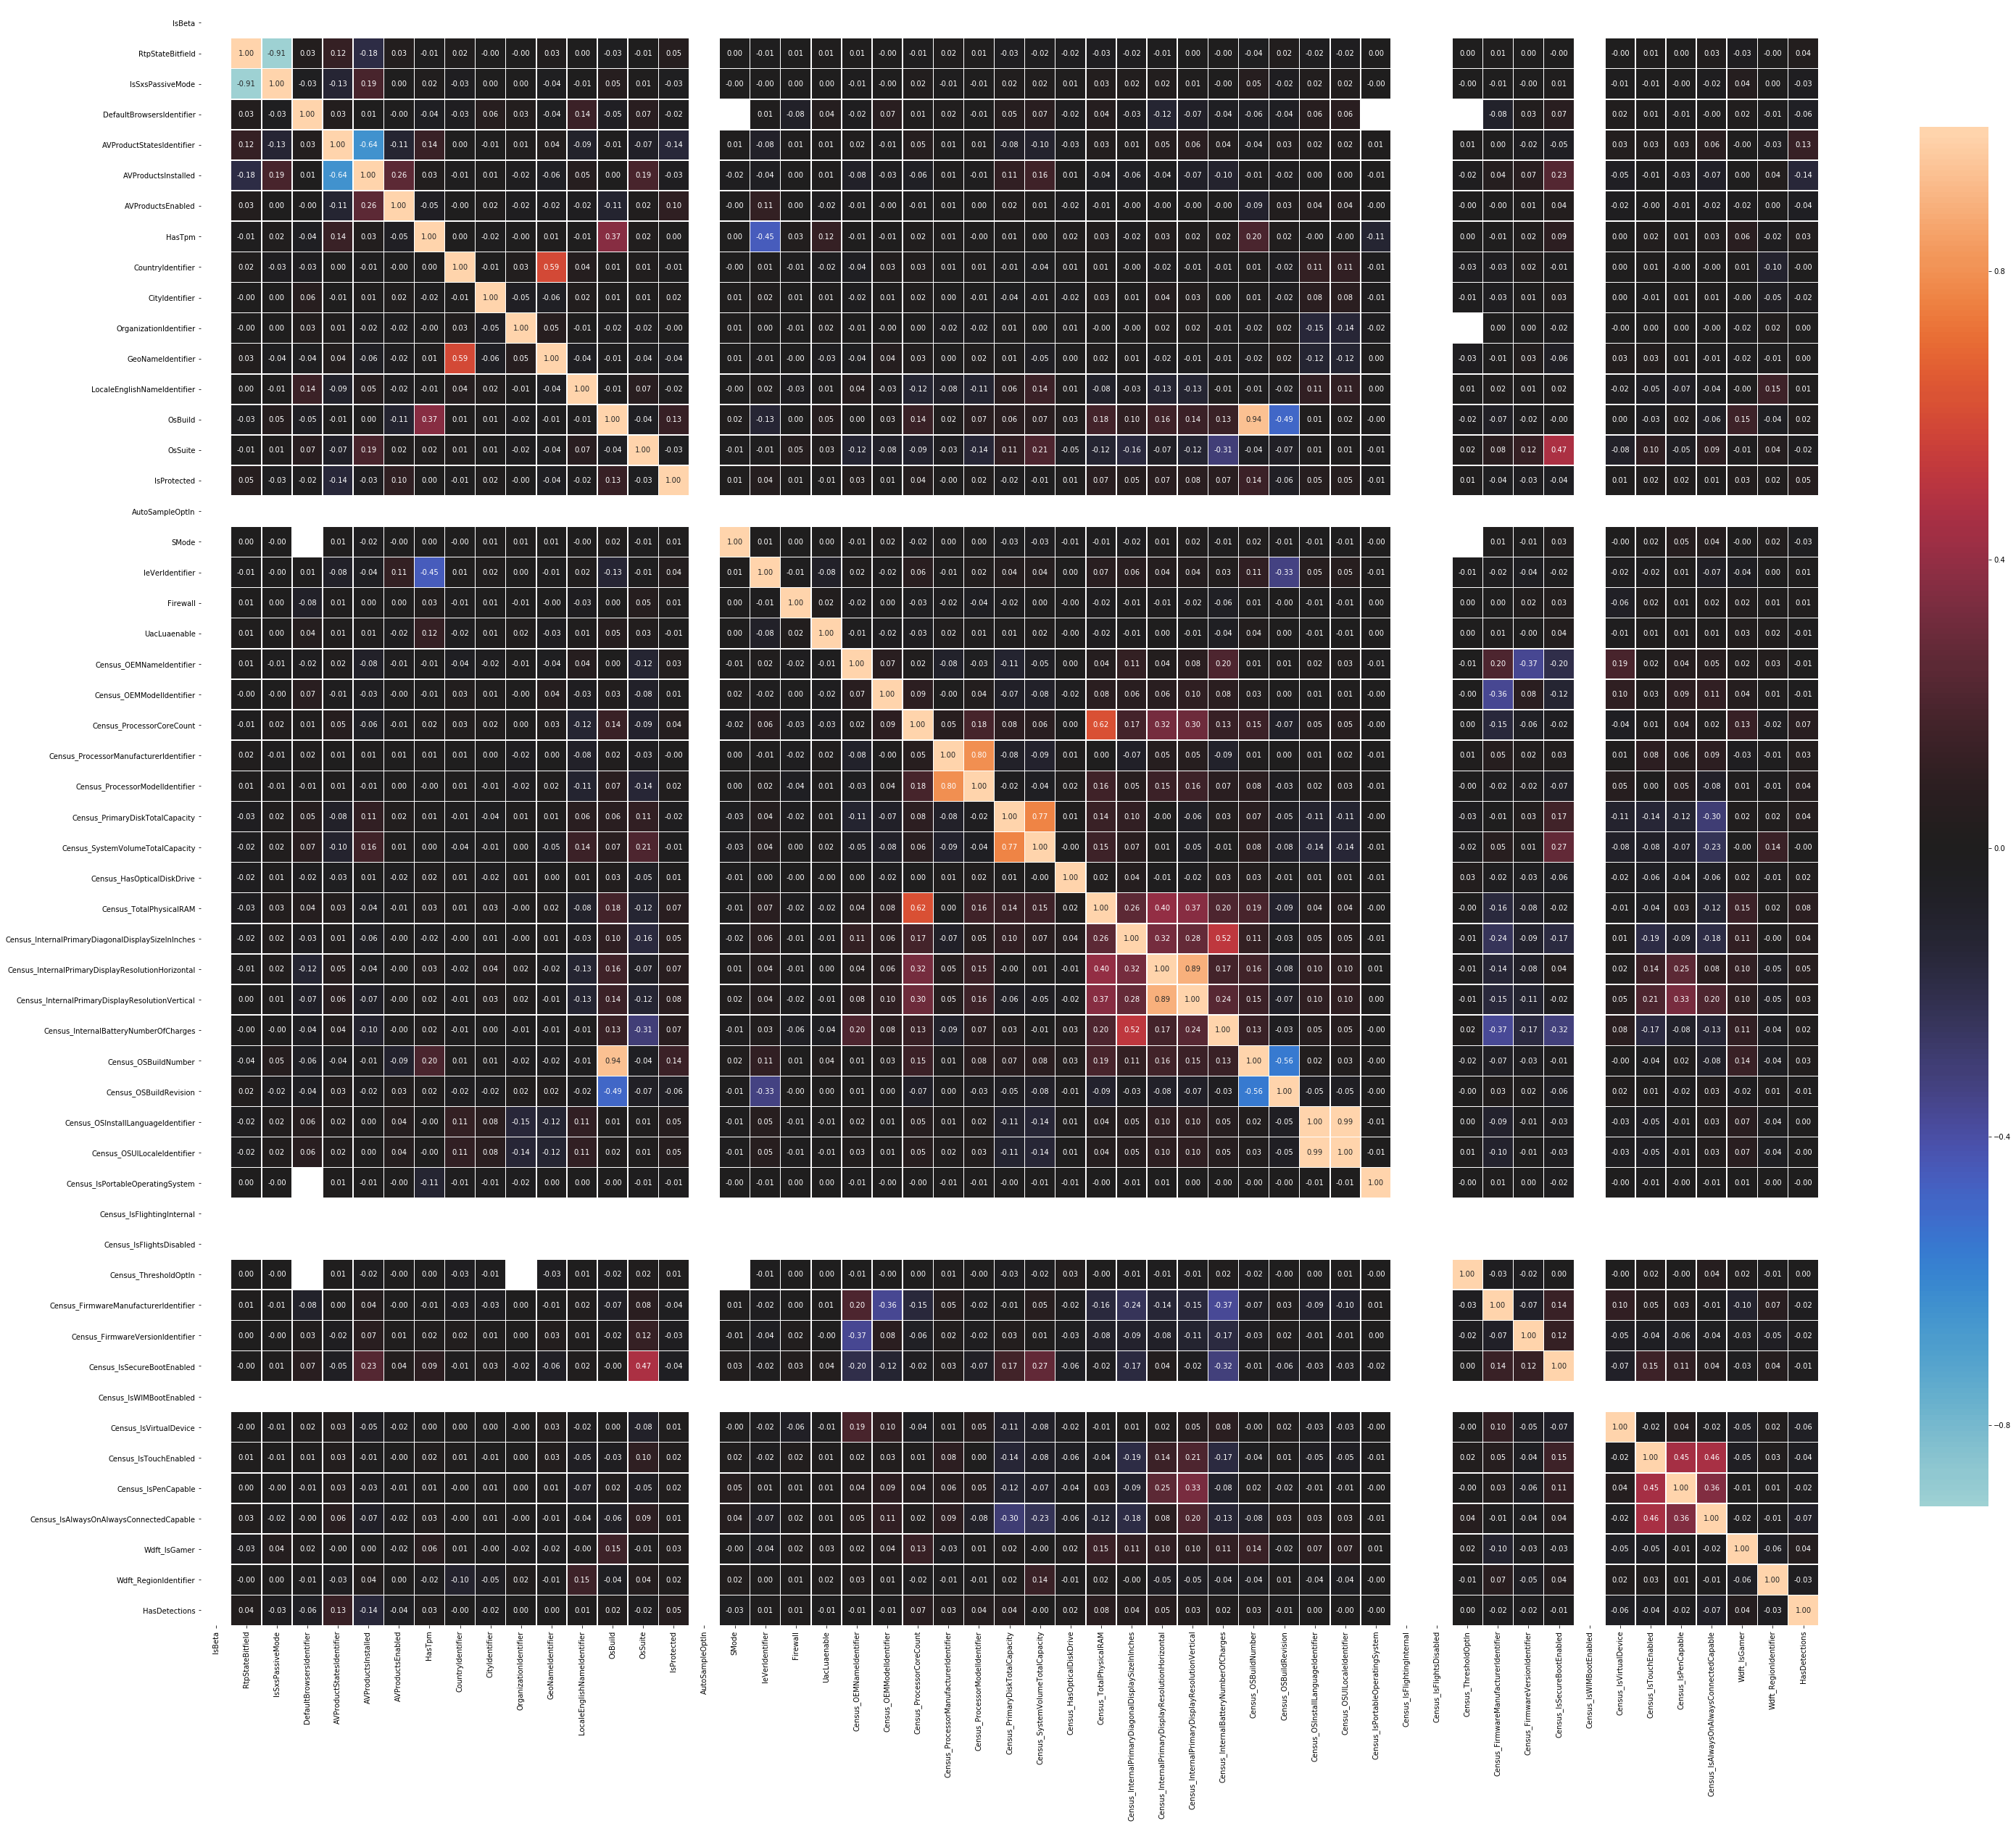
\includegraphics[scale=0.2]{correlation.PNG}

% that's all folks

\end{document}


